\documentclass[12pt]{article}
\usepackage{pdfpages}
\usepackage{xcolor}

\usepackage{setspace}
\onehalfspacing
\usepackage[a4paper, margin=1in]{geometry}

\title{Case Study 2 - Product Liability}
\author{Graham Pellegrini }
\date{\today}

\begin{document}

\maketitle

\section{Question 1}
\textbf{Were the GM engineers responsible for the problems with the Cadillac Seville and Deville models? (Yes vs No debate – if no, who was responsible?)}

\begin{itemize}
    \item [\textcolor{blue}{Yes}] GM engineers were aware that the cars exceeded EPA emission limits.
    \item [\textcolor{blue}{Yes}] Regardless of management pressure, they had a professional duty and the opportunity to whistleblow.
    \item [\textcolor{red}{No}] The engineers followed company directives and did not directly decide to manipulate emissions.
    \item [\textcolor{red}{No}] Regulations did not explicitly prohibit non-climate-controlled testing, and the EPA failed to enforce stricter measures.
    \item [\textcolor{blue}{Yes}] The engineers used testing methods that did not reflect real-world conditions, intentionally misleading the EPA.
    \item [\textcolor{red}{No}] There was no clear legal obligation preventing the engineers from following instructions that where given to them.
    \item [\textcolor{blue}{Yes}] Other companies also bypassed regulations, and the form of cheating the system was common practice in the industry.
    \item [\textcolor{blue}{Yes}] The effort spent devising a workaround could have been used to develop a legitimate solution.
    \item [\textcolor{blue}{Yes}] Engineers, given their expertise, have a responsibility to ensure products are safe and compliant with regulations.
    \item [\textcolor{red}{No}] In corporate environments, directives may be unclear, and engineers might lack full knowledge of the situation.
    \item [\textcolor{red}{No}] Compliance is management's responsibility; engineers are expected to work within the provided framework.
    \item [\textcolor{blue}{Yes}] Engineers who implemented the bypass had the technical knowledge to understand the ethical and legal consequences.
    \item [\textcolor{blue}{Yes}] They have a duty to protect both the environment and public safety.
    \item [\textcolor{red}{No}] Engineers also have contractual obligations to their employer and must follow company directives.
\end{itemize}

\section{Question 2}
\textbf{Read about the recent Volkswagen emissions Scandal (2015). Were the engineers responsible when faced with the problem that their cars were not adhering to emission standards. (Yes vs No debate. If not who was responsible, if yes what should they have done?)}

\begin{itemize}
    \item [\textcolor{red}{No}] Modern corporate culture prioritizes output, creating pressure to meet market demands.
    \item [\textcolor{blue}{Yes}] The software was deliberately designed to cheat the system, and engineers were held responsible.
    \item [\textcolor{red}{No}] Weak oversight by governing bodies responsible for auditing companies.
    \item [\textcolor{red}{No}] Engineers cannot be blamed, as their work is heavily driven by production demands.
    \item [\textcolor{red}{No}] Their role was simply to meet targets, regardless of the means.
    \item [\textcolor{blue}{Yes}] Regulators cannot be blamed since the software was explicitly designed to bypass regulations.
    \item [\textcolor{blue}{Yes}] The intentional nature of the cheat undermines the professionalism of the engineers involved.
    \item [\textcolor{red}{No}] Volkswagen had to protect its reputation, and managers put engineers in a difficult position.
    \item [\textcolor{red}{No}] Engineers had limited influence over design and decision-making within the company.
    \item [\textcolor{blue}{Yes}] They could have formed an internal group to address the ethical concerns of the software.
    \item [\textcolor{blue}{Yes}] In hindsight, the issue damaged the company further; speaking up earlier could have prevented this.
    \item [\textcolor{blue}{Yes}] Engineers should have sought an alternative solution rather than compromising their integrity and reputation.
    \item [\textcolor{red}{No}] Other companies likely use similar systems, but their actions remain undisclosed.
    \item [\textcolor{blue}{Yes}] The fact that competitors engage in the same practice does not justify it.
    \item [\textcolor{blue}{Yes}] Innovation is key in engineering, yet they opted for a workaround instead of a real solution.
    \item [\textcolor{red}{No}] Engineers work within the constraints given by management, which limits their ability to innovate.
\end{itemize}

\section{Question 3}
\textbf{Is it appropriate to use data such as these in Ford’s decision regarding whether or not to make a safety improvement in its engineering design. What responsibilities do you think engineers have in situations like this?  (Group A Yes vs Group B No debate)}

\begin{itemize}
    \item [\textcolor{red}{No}] Engineers, bound by their professional Code of Conduct and Ethics, cannot put a price on human life.
    \item [\textcolor{blue}{Yes}] The company was conducting a risk assessment. It is not always possible to make a product 100\% safe.
    \item [\textcolor{blue}{Yes}] Cost-benefit analysis is a standard practice across industries. For example, the food industry weighs the costs of using certain ingredients or chemicals. Since businesses aim to be profitable, the cost of implementing safety features must be considered.
    \item [\textcolor{blue}{Yes}] If every possible safety feature were included in a car, costs would be so high that consumers could not afford it. Additionally, competition allows consumers to choose safer alternatives from other manufacturers.
    \item [\textcolor{red}{No}] It is inhumane to put a price on suffering and death. Moreover, such values are questionable, especially if companies profit from them.
    \item [\textcolor{blue}{Yes}] Cost-benefit analysis is a common and necessary practice in business.
    \item [\textcolor{red}{No}] The company saved only \$11 per car by not implementing the safety feature—a small price to pay for consumer safety.
    \item [\textcolor{blue}{Yes}] The issue was identified during testing and made public. Ultimately, it was the consumer's choice to purchase the car.
    \item [\textcolor{red}{No}] Not all consumers conduct extensive research and may be unaware of the risks. Furthermore, car dealers prioritize sales and may not disclose potential dangers.
    \item [\textcolor{blue}{Yes}] The company did not violate any regulations. Stricter policies should have been in place to prevent such situations.
    \item [\textcolor{blue}{Yes}] Cost-benefit analysis is a standard business practice. However, such assessments are typically internal documents and not disclosed to the public.
\end{itemize}

\section{Question 4}
\textbf{Were the design engineers right to refuse to look at the lifting plans? Should they have recommended that the riggers consult a specialist?  (Group A Yes vs Group No debate)}

\begin{itemize}
    \item [\textcolor{blue}{Yes}] The engineers had the right to refuse, as it was not their contractual responsibility to determine how to rig the tower.
    \item [\textcolor{red}{No}] Ethical concerns arise, especially since lives were lost. The engineers should have at least reviewed the plans and issued a warning.
    \item [\textcolor{blue}{Yes}] If there was no contractual obligation and the engineers were explicitly ordered not to review the plans—especially considering past similar incidents—then they were justified in refusing.
    \item [\textcolor{blue}{Yes}] The riggers were not solely dependent on the engineers' expertise; they could have consulted external specialists.
    \item [\textcolor{red}{No}] The engineers witnessed the riggers struggling and took no action to assist them.
    \item [\textcolor{red}{No}] The riggers were unable to proceed as intended since the top part of the tower was marked as non-removable. However, after that restriction was set, no further instructions were provided.
    \item [\textcolor{red}{No}] Due to the custom nature of the design, certain aspects could only have been explained by the engineers.
    \item [\textcolor{blue}{Yes}] Documentation exists precisely for this reason—to avoid relying on engineers' direct involvement. The necessary design details should have been outlined in those documents.
    \item [\textcolor{blue}{Yes}] Since the riggers consulted the engineers and it was evident they lacked the knowledge to rig the tower, they should have sought a specialist, as rigging was ultimately their responsibility.
\end{itemize}

\section{Question 5}
\textbf{Was Judge Wolverton’s judgement appropriate? How relevant is it that subsequent review showed that none of the falsified documents needed to be changed?  (Group A Yes vs Group B No debate.)}

\begin{itemize}
    \item [\textcolor{blue}{Yes}] The judge's decision was appropriate, as falsifying documents is a serious offense that violates the trust placed in engineers. While it may expedite processes, it is unethical.
    \item [\textcolor{blue}{Yes}] Without the judge's ruling, the case could have set a dangerous precedent and reinforced a harmful mentality.
    \item [\textcolor{red}{No}] The falsified documents did not impact the final outcome and would have been justified if they had been legitimate. The judge's decision was overly harsh.
    \item [\textcolor{blue}{Yes}] While no immediate harm resulted from this case, the judge's decision was necessary to deter future incidents with potentially severe consequences.
    \item [\textcolor{blue}{Yes}] The engineers whose names were falsely used on the documents were also affected, and the judge had to consider their involvement.
    \item [\textcolor{red}{No}] Apart from the falsification, the work was completed correctly, and no harm was done.
    \item [\textcolor{blue}{Yes}] Given how the court system operates, justifying document falsification would have set a precedent for future cases that could have led to more severe consequences.
\end{itemize}

Note: I was in the "Yes" group, and I thought that the opposing "No" group could have argued that the judge's decision was actually not harsh enough (i.e., it was appropriate but too lenient). Since 40 documents were falsified and only 20 days of prison were assigned, this implies that one could falsify a document in a serious case and receive only 0.5 days of prison per document. I would have taken a different stance if I were in the "No" group.
\footnote{The use of ChatGPT (AI Model used) was limited to the extent stated in the report.}
\pagebreak

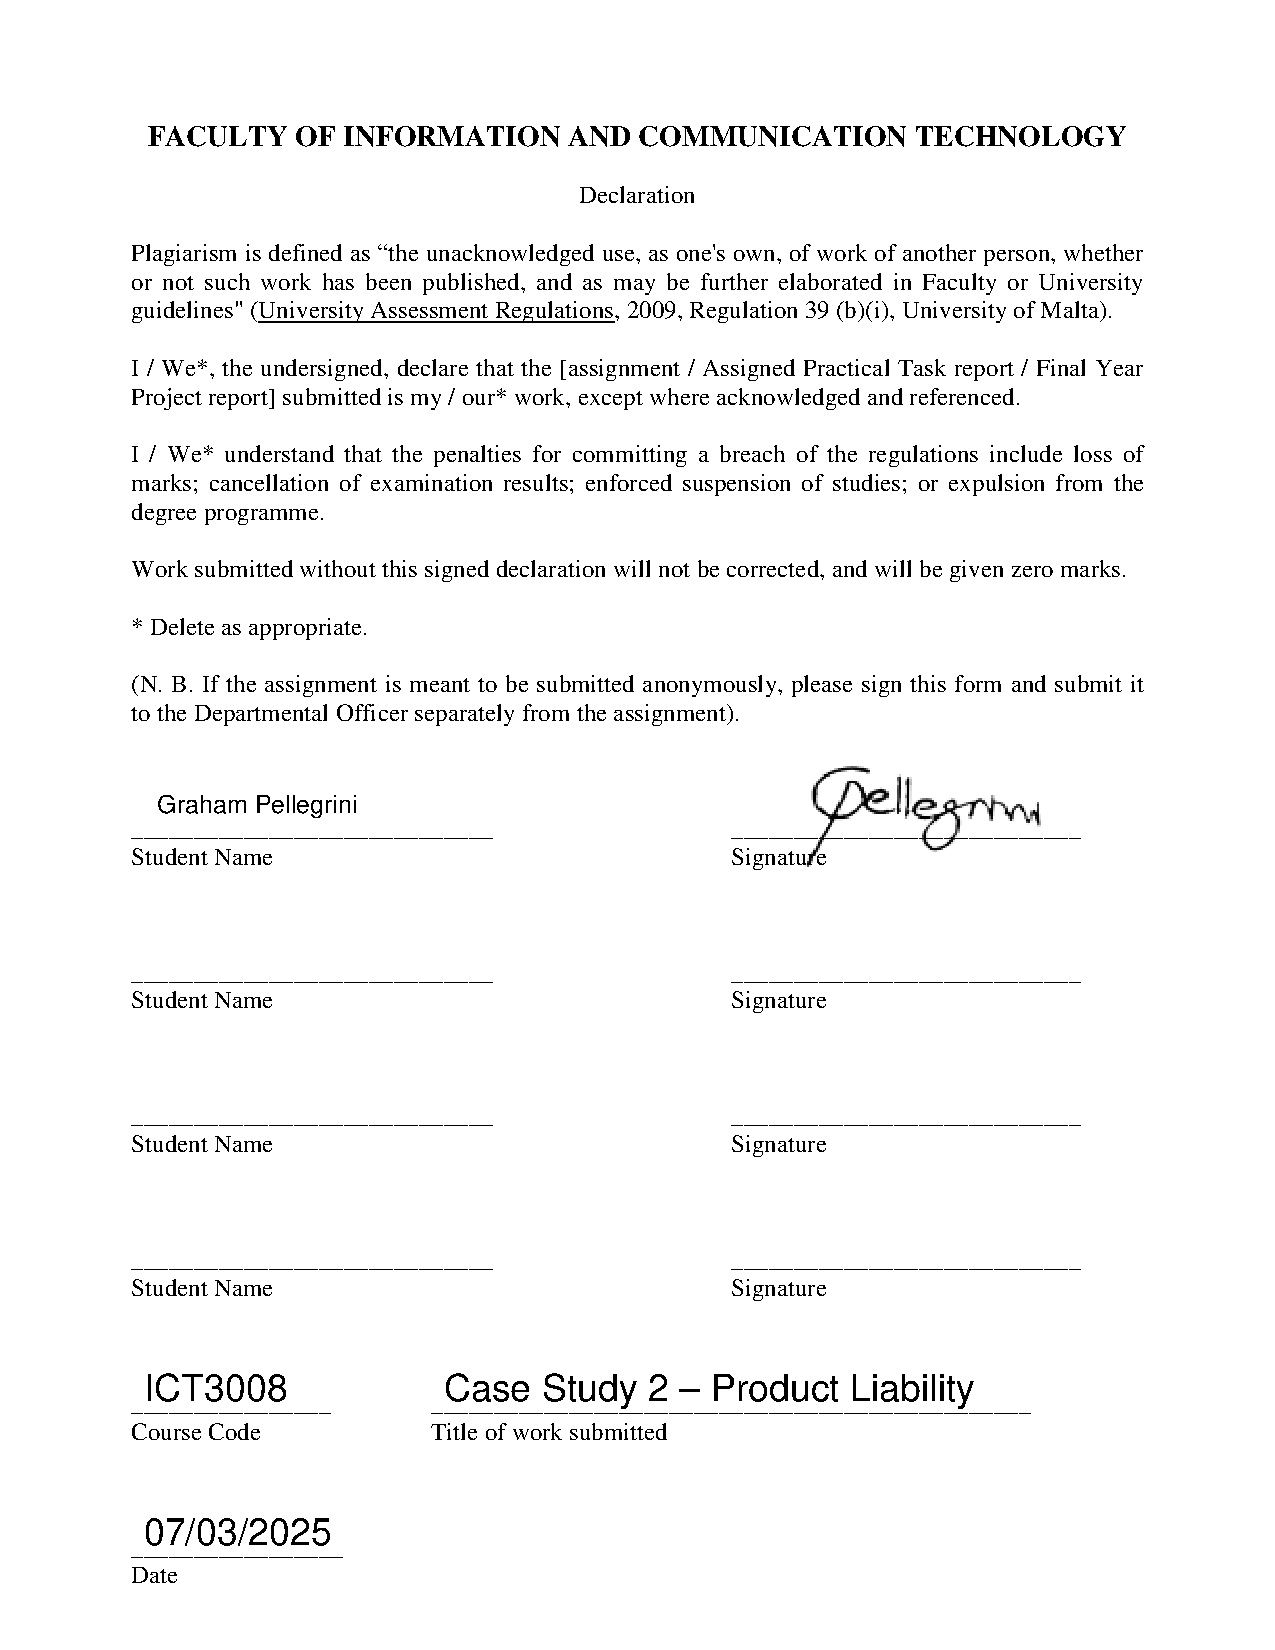
\includepdf[pages=-]{Plagiarism_Declaration_Form.pdf}

\end{document}
